\subsubsection{Context}

Conventional systems neuroscience experiments are typically short in duration
and often place significant constraints on subject behaviour to simplify data
analysis.
%
However, these restrictions may limit our ability to observe critical
aspects of brain function and behaviour that only manifest in more naturalistic
and extended conditions.

At the Sainsbury Wellcome Centre (SWC) and Gatsby Computational Neuroscience
Unit (GCNU) we are pioneering Naturalistic, Long-Duration, and Continual
(NaLoDuCo) foraging experiments in mice that span weeks to months. During these
experiments, we collect high-resolution behavioural and neural recordings in
naturalistic settings.
%
% The data generated by these experiments creates unprecedented challenges for
% their characterization, so we are building novel analytical methods addressing
% these challenges.

This novel experimental approach will enable researchers to explore neural
mechanisms underlying naturalistic behaviour over extended periods for the first
time, offering the possibility of uncovering insights across a wide range of
phenomena, including long-term behavioural adaptation, neural plasticity, and
learning.
%
The data generated from NaLoDuCo experiments represent an entirely new resource
in neuroscience, with the potential to drive breakthroughs and discoveries that
are beyond the reach of traditional experiments.

Our US collaborator, the Allen Institute for Neural Dynamics (AIND) is also investigating
foraging, but using head-fixed mice. Key to their mission is distributing very large Neuroscience datasets,
and providing functionality to process them on the cloud.

Our UK business partner, NeuroGEARS Ltd.\ has been a key business partner of the SWC for the
implementation of the NaLoDuCo experimental framework since the project started
in 2021, and also provides services to the AIND.

Together we aim at empowering research centres worldwide to adopt this groundbreaking
approach.
%
However, the extremely large datasets--on the order of hundreads of terabytes--
gathered from experiments spanning weeks to months pose significant
challenges in data acquisition, visualisation, and analysis.

While experiments in neuroscience that are naturalistic, long-duration, or
continuous have been conducted in the past
\citep[e.g.,][]{jhuangEtAl10,maoEtAl21,volohEtAl23}, to the best of our
knowledge, we are the first to integrate all three of these features in a
single experimental paradigm.
%
This combination introduces unprecedented complexities in data processing, as
we aim to capture behaviour and brain activity in their most ecologically valid,
extended, and uninterrupted forms.

Here we will address these complexities by sharing openly expertise
and building software infrasctructure to enable this transformative type of
experimentation.

\subsubsection{Focus areas}

The focus areas of the proposed project are (Figure~\ref{fig:focusAreas}):

\begin{description}

    \item[Data Collection \& Management] Efficiently gathering and organising
        massive datasets over extended periods.

    \item[Data Sharing] Providing global access to large-scale datasets.

    \item[Data Visualisation] Developing efficient web-based tools to visualise
        very large behavioural and neural datasets.

    \item[Spike Sorting] Assigning spikes to neurons reliably and tracking
        individual neurons across long-periods of time in real time.

    \item[Data Analysis] Characterising behavioural and neural recordings
        (Figure~\ref{fig:dataAnalysis}).

    \item[Inference-Driven Experimentation] Creating a new type of
        experimentation driven by real-time behavioural and neural inferences.

\end{description}

\begin{figure}
    \begin{center}
        \resizebox{4.0in}{!}{%
            \resizebox{5in}{!}{%
    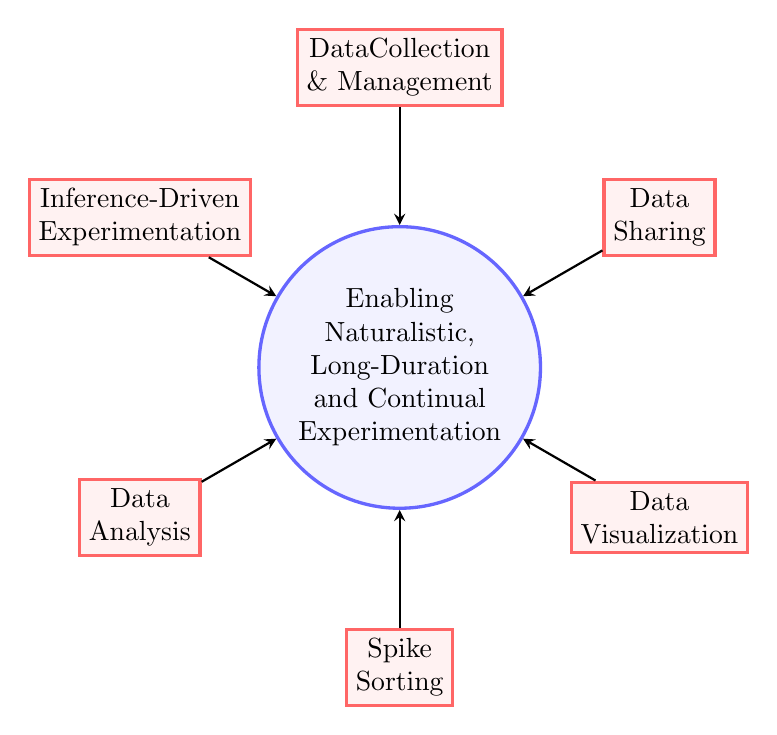
\begin{tikzpicture}[
            node distance=4cm and 1cm,
            centralNode/.style={circle, draw=blue!60, fill=blue!5, very thick,
            minimum size=7mm, align=center},
            itemNode/.style={rectangle, draw=red!60, fill=red!5, very thick,
            minimum size=5mm, align=center},
            arrow/.style={thick, <-, >=stealth},
        ]
        \node[centralNode] (naloducoExp)    {Enabling\\Naturalistic,\\Long-Duration\\and Continual\\Experimentation};
        % \node[itemNode]    (dataCol)        at (naloducoExp) ++(40:2cm) {DataCollection\\\& Management};
            \path (naloducoExp) ++(90:1.5in) node[itemNode] (dataCol) {DataCollection\\\& Management};
            \path (naloducoExp) ++(30:1.5in) node[itemNode] (dataSharing) {Data\\Sharing};
            \path (naloducoExp) ++(330:1.5in) node[itemNode] (dataVis) {Data\\Visualization};
            \path (naloducoExp) ++(270:1.5in) node[itemNode] (spikeSort) {Spike\\Sorting};
            \path (naloducoExp) ++(210:1.5in) node[itemNode] (dataAnalysis) {Data\\Analysis};
            \path (naloducoExp) ++(150:1.5in) node[itemNode] (inferenceDExp) {Inference-Driven\\Experimentation};
        \draw[arrow] (naloducoExp) -- (dataCol);
        \draw[arrow] (naloducoExp) -- (dataSharing);
        \draw[arrow] (naloducoExp) -- (dataVis);
        \draw[arrow] (naloducoExp) -- (spikeSort);
        \draw[arrow] (naloducoExp) -- (dataAnalysis);
        \draw[arrow] (naloducoExp) -- (inferenceDExp);
    \end{tikzpicture}
}

        }
    \end{center}
    \caption{Project theme (blue) and focus areas (red).}
    \label{fig:focusAreas}
\end{figure}

\begin{figure}
    \centering
    \subfloat[]{
        \resizebox{3.0in}{!}{%
            \begin{tikzpicture}[
        node distance=4cm and 1cm,
        behaviorNode/.style={ellipse, draw=cyan!60, fill=cyan!5, very thick,
        minimum size=7mm, align=center},
        problemNode/.style={rectangle, draw=gray!60, fill=gray!5, very thick,
        minimum size=5mm, align=center},
        arrow/.style={thick, <-, >=stealth},
    ]
    \node[behaviorNode] (behavior)    {Behavior};
        \path (behavior) ++(190:1.0in) node[problemNode] (mbpTracking) {Multi\\Body Part\\Tracking};
        \path (behavior) ++(230:1.0in) node[problemNode] (kinematicsInference) {Kinematics\\Inference};
        \path (behavior) ++(310:1.0in) node[problemNode] (statesInference) {State\\Inference};
        \path (behavior) ++(350:1.0in) node[problemNode] (policyInference) {Policy\\Inference};
    \draw[arrow] (behavior) -- (mbpTracking);
    \draw[arrow] (behavior) -- (kinematicsInference);
    \draw[arrow] (behavior) -- (statesInference);
    \draw[arrow] (behavior) -- (policyInference);
\end{tikzpicture}

        }
    }
    \hfill
    \subfloat[]{
        \resizebox{2.25in}{!}{%
            \begin{tikzpicture}[
        node distance=4cm and 1cm,
        neuralNode/.style={ellipse, draw=magenta!60, fill=magenta!5, very thick,
        minimum size=5mm, align=center},
        problemNode/.style={rectangle, draw=gray!60, fill=gray!5, very thick,
        minimum size=5mm, align=center},
        arrow/.style={thick, <-, >=stealth},
    ]
    \node[neuralNode] (neural)    {Neural\\Activity};
        \path (neural) ++(190:1.0in) node[problemNode] (spikeSorting) {Spike\\Sorting};
        \path (neural) ++(230:1.0in) node[problemNode] (latentsInference) {Latents\\Inference};
        \path (neural) ++(310:1.0in) node[problemNode] (stateInference) {State\\Inference};
        \path (neural) ++(350:1.0in) node[problemNode] (decoding) {Decoding};
    \draw[arrow] (neural) -- (spikeSorting);
    \draw[arrow] (neural) -- (latentsInference);
    \draw[arrow] (neural) -- (stateInference);
    \draw[arrow] (neural) -- (decoding);
\end{tikzpicture}

        }
    }
    \caption{Behavioural (a) and neural (b) data analysis problems to address.}
    \label{fig:dataAnalysis}
\end{figure}

\subsubsection{Cross fertilisation}

The foraging experiments at the AIND are different from those at the SWC. They
do not probe freely moving and naturalistic behaviour, but are able to perform
electrophysiological recordings more densely than those at the SWC.
%
These experimental approaches to foraging are complementary and this
collaboration will greatly benefit both of them.

At the GCNU and the AIND we are independently developing methods to address
several of the focus areas in Figure~\ref{fig:focusAreas}. We will join forces
to codevelop these areas and our foraging research programs.
